\chapter{Neural Network Detectors}
\todo{bla}
NNs vs ML

\section{Precision Metrics}
mAP, IoU

\section{Classification networks}
\label{chapt:cnets}
In order to better understand the detection networks, we will shortly describe their predecessors, classification networks. Classification network is a convolutional neural network (CNN) \cite[ch.~9]{bib:dlbook} that given an image, returns a confidence score of correspondence to each of the classes. Usually \textit{soft-max} function is applied to the confidence score to represent probability distribution.

In \cref{chapt:models} we will show how classification models are used as a backbone for the detectors.

\subsection*{AlexNet (2012)}
A significant breakthrough in use of CNNs happened in 2012, when the \textit{AlexNet} \cite{bib:alexnet} won the \textit{ImageNet} image recognition challenge\footnote{\url{http://www.image-net.org/challenges/LSVRC/}}. It was the first time a deep CNN performed better than traditional computer vision and machine learning approaches. 

AlexNet has a simple architecture with five convolutional layers and two fully connected layers followed by a softmax layer. It created a foundation on which today's state-of-the-art models are build and set a new standard for the image recognition.

\subsection*{VGG (2014)}
\label{sec:VGG}
The network architecture, mostly known as VGG \cite{bib:vgg}, pushed the concept of AlexNet even further and proved the feasibility of deeper network with small convolutions. 

Each of the VGG's convolutional filters uses 3 by 3 kernel and the depth of the filters increases thought the network, reaching 512 filters in the last layers. After the convolutions, three fully connected layers and softmax are applied, see \cref{tab:vggarch}. There are multiple versions of the VGG architecture, depending on the number of convolutional layers, the most popular is 16 layer version. 

VGG network is considered a general architecture for a classifier network due to it's linear architecture with decreasing size of the features and increasing number of channels. 

\begin{table}[]
    \centering
    \rotatebox{90}{
        \vggArch
    }
    \caption{Architecture of VGG network, version D. Taken from \cite[table 1]{bib:vgg}}
    \label{tab:vggarch}
\end{table}
    
\subsection*{Inception (v1) (2014)}
\label{sec:inception}
Previous architectures showed that increasing the number of layers and layer size leads to better precision. Inception v1 \cite{bib:googlenet}, also known as GoogLeNet, aims at increasing precision while improving utilization of computing resources.

In order to avoid the growing cost of stacking more layers, the network introduces the concept of sparsity, by using the \textit{inception modules} \cref{fig:incept_mod}. The sparse structure is approximated by dense components using multiple convolutions with different kernel sizes and concatenating the outputs together. Max-pooling is also performed as an alternative to convolutions and concatenated to the module output. The computational cost of convolutions is lowered by a dimensionality reduction of channels, introduced in the form of preceding 1 by 1 convolutions. The network is then formed by linearly stacking nine inception modules, preceded by a linear stem network and followed by a fully connected classifier. 

\paragraph{Inception v2} bla

\paragraph{Inception v3} bla

\paragraph{Inception v4} bla


\begin{figure}
    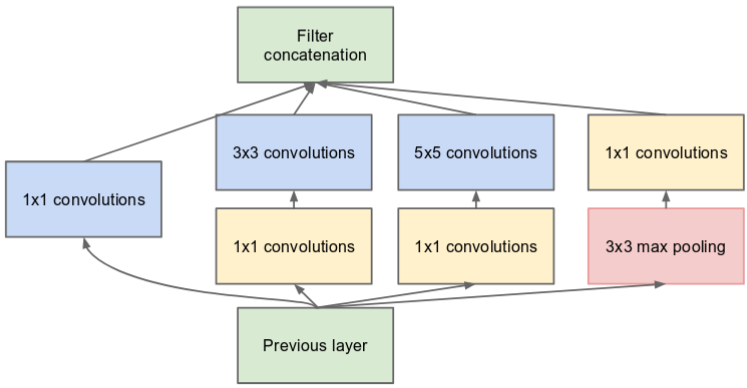
\includegraphics[width=\textwidth]{img/inception}
    \caption{Inception module, picture from \cite[figure 2]{bib:googlenet}.}
    \label{fig:incept_mod}
\end{figure}

\subsection*{ResNet (2015)}
\label{sec:resnet}
\todo{desc resnet}

All ResNet \cite{bib:resnet} architectures (ResNet-10, ResNet-18, 34, 50...) use the same architecture (left chart), which is build from a few input layers, four sets of building blocks and output layers. Each of four blocks can be composed of multiple residual building blocks. There are two types of building blocks, larger block with three convolutional layers called "bottleneck", or smaller "basic" block with two convolutional layers.  see \cref{fig:resnet_arch}

\paragraph{Inception-ResNet}

\begin{figure}
    \resnetArch
    \caption{Architecture of ResNet network.
    Note that the give number of convolutional filters in building blocks depends on which block do they belong to. For more detailed specification see Table 1 in  \cite{bib:resnet}.}
    \label{fig:resnet_arch}
\end{figure}

\subsection*{Present day networks}
 comparing \cref{fig:cnncomp}

\begin{figure}
    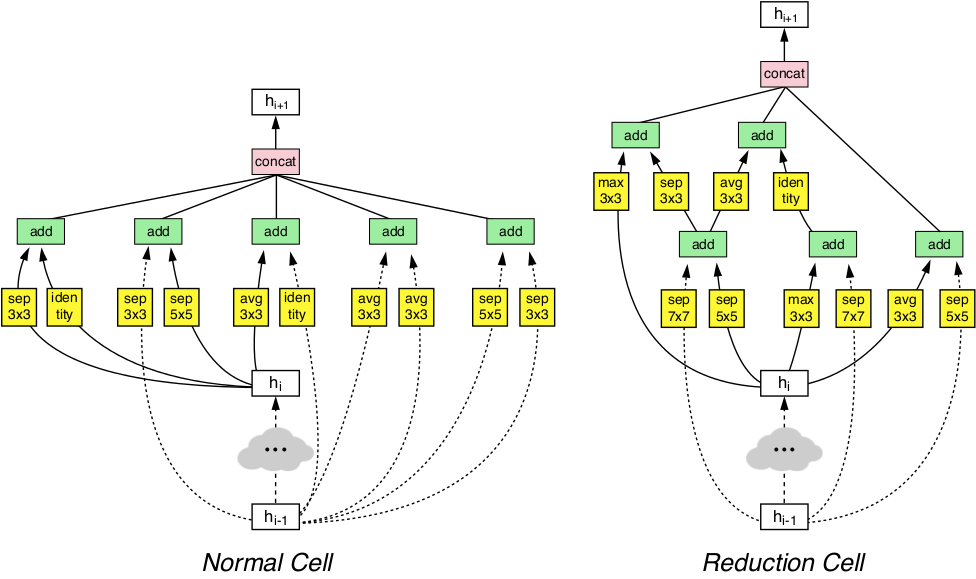
\includegraphics[width=\textwidth]{img/nasnet}
    \caption{Accuracy versus computational demand across top performing published CNN architectures on ImageNet 2012 ILSVRC challenge prediction task. Computational demand is measured in the number of floating-point multiply-add operations to process a single image. Taken from \cite{bib:nasnet}.}
    \label{fig:cnncomp}
\end{figure}

\todo{add comp table for all models}

\section{Detection networks}
\label{chapt:models}

\todo{bla}

\subsection*{Region-based Convolutional Network (R-CNN)}
\subsubsection{R-CNN}
\subsubsection{Fast R-CNN}
\subsubsection{Faster R-CNN}

\subsection*{Mask Region-based Convolutional Network (Mask R-CNN)}

\subsection*{You Only Look Once (YOLO)}
\subsubsection{YOLO}
\label{sec:yolo}
\subsubsection{YOLO v2 and YOLO 9000}

\subsection*{Single-Shot Detector (SSD)}
\label{sec:ssd}
\subsubsection{SSD}

\subsubsection{FSSD}
\subsubsection{RFB}


\section{Use of Detection networks for video processing}

%Optional section
% \section{Other uses of CNNs}
% \subsection{Noise removal/ Regularization}
% \subsection{Image generation}





